\documentclass[12pt]{article}
\usepackage{amsmath}
\usepackage{graphicx}
\usepackage{enumerate}
\usepackage{natbib}
\usepackage[T1]{fontenc}
\usepackage[latin9]{inputenc}
\usepackage{color}
\usepackage{float}
\usepackage{hyperref}
\usepackage{multirow}
%\usepackage{babel}

\newcommand{\blind}{0}

\addtolength{\oddsidemargin}{-.75in}%
\addtolength{\evensidemargin}{-.75in}%
\addtolength{\textwidth}{1.5in}%
\addtolength{\textheight}{1.3in}%
\addtolength{\topmargin}{-.8in}%

\makeatletter

%%%%%%%%%%%%%%%%%%%%%%%%%%%%%% LyX specific LaTeX commands.
%% Because html converters don't know tabularnewline
\providecommand{\tabularnewline}{\\}

\newcommand{\red}[1]{{\color{red} #1}}

\makeatother

\begin{document}

\begin{center}
{\large\bf Appendices to}\\
\vspace{0.2cm}
{\LARGE\bf Enabling Interactivity on Displays of Multivariate
Time Series and Longitudinal Data}\\
\vspace{0.3cm}
{\large\bf published in the Journal of Computational and Graphical Statistics}
\end{center}
\addcontentsline{toc}{section}{\appendixname}
\renewcommand{\thesection}{\Alph{section}}
\setcounter{table}{0}
\renewcommand{\thetable}{C\arabic{table}}
\setcounter{figure}{0}
\renewcommand{\thefigure}{C\arabic{figure}}

\section{Wrapping}\label{sub:appendix-wrapping}

Recall that $\Delta_{n-j}=x_{(n-j)}-x_{(1)}+1$,
then the new $x$-coordinate after $j$ keystrokes
for $x$-wrapping, $x^*$ of $x$ is
\begin{eqnarray*}
x^* & = & \begin{cases}
x_{(n-j)}  & \mbox{if~} x-x_{(1)}+1 \mbox{~mod}\Delta_{n-j} = 0\\
(x-x_{(1)}+1) \mbox{~mod}\Delta_{n-j} ~~+x_{(1)}-1 &  \mbox{o.w.}
\end{cases} \\
& = & \begin{cases}
x_{(n-j)}  & \mbox{if~} (x-x_{(1)}+1) \mbox{~mod}\Delta_{n-j} = 0\\
(x-x_{(1)}+1)-\left\lfloor\frac{x-x_{(1)}+1}{\Delta_{n-j}}\right\rfloor\times\Delta_{n-j}+x_{(1)}-1 &\mbox{o.w.}\\
\end{cases} \\
 & = &
(x-x_{(1)}+1)-\left(\left\lceil\frac{x-x_{(1)}+1}{\Delta_{n-j}}\right\rceil -1\right)\times \Delta_{n-j} +x_{(1)}-1 \\ & = &
x-\left(\left\lceil \frac{x-x_{(1)}+1}{\Delta_{n-j}}\right\rceil -1\right)\times\Delta_{n-j},
\end{eqnarray*}
enabling the movements for $i=$ wrap to be described as
\begin{eqnarray*}
\mathbf{m}{}_{ij} & = & \begin{cases}
(-\left(\left\lceil \frac{\mathbf{x}-x_{(1)}+1}{\Delta_{n-j}}\right\rceil -1\right)\times\Delta_{n-j}, \; 0) & 1\leq j \leq n-3 \\
(-\left(\left\lceil \frac{\mathbf{x}-x_{(1)}+1}{\Delta_3}\right\rceil -1\right)\times\Delta_3, \; 0) & j\ge n-2
\end{cases} \\
\end{eqnarray*}
or equivalently in terms of line group indicators as well as points as
\begin{eqnarray*}
\mathbf{m}{}_{ij} & = & \begin{cases}
(-(\mathbf{l}{}_{ij} -1)\times\Delta_{n-j}, \; 0) & 1\leq j \leq n-3 \\
(-(\mathbf{l}{}_{ij} -1)\times\Delta_3, \; 0) & j\ge n-2.
\end{cases}
\end{eqnarray*}
The line group indicator $\mathbf{l}{}_{ij}$ will depend on
the number of interactions $j$.

Sometimes it is useful to wrap the series faster. If you have
a long time series, it might be useful to make full year jumps.
This can be achieved with the above equations by setting the
sequence of $j$ to respect this period. In other instances it
may be useful to have a multiplicative wrapping so that it
looks like the series wraps faster and faster with each step.
That means every keystroke will send a different number of
points from the right to the left. The number of points
wrapped by the $j$th step, can be represented by the user
input parameter $u_{ij}$. Then the $x$-range after $j$ steps
is $(x_{(1)}, x_{(n-\sum_{a=1}^j u_{ia})})$, yielding
$\Delta_{n-\sum_{a=1}^j u_{ia}}=x_{(n-\sum_{a=1}^j u_{ia})}-x_{(1)}+1$, and
\begin{eqnarray*}
x^* & = & x-\left(\left\lceil \frac{x-x_{(1)}+1}{\Delta_{n-\sum_{a=1}^j u_{ia}}}\right\rceil -1\right)\times\Delta_{n-\sum_{a=1}^j u_{ia}}, \\
\mathbf{m}{}_{ij} & = & \begin{cases}
(-(\mathbf{l}{}_{ij} -1)\times\Delta_{n-\sum_{a=1}^j u_{ia}}, \; 0) & 1\leq \sum_{a=1}^j u_{ia} \leq n-3 \\
(-(\mathbf{l}{}_{ij} -1)\times\Delta_3, \; 0) & \sum_{a=1}^j u_{ia}\ge n-2.
\end{cases}
\end{eqnarray*}

If the user wants to skip all intermediate positions and use
only one jump to the fully wrapped position, %as shown in Figure
%\ref{fig:faceting-period} from the left to center panel,
then the new $x$-range will be $(x_{(1)}, x_{(p_{i2})})$, where
the parameter $p_{i2}$ is the length of period. Hence for $j\ge 1$,
\begin{eqnarray*}
x^* & = & x-\left(\left\lceil \frac{x-x_{(1)}+1}{\Delta_{p_{i2}}}\right\rceil -1\right)\times\Delta_{p_{i2}}, \\
\mathbf{m}{}_{ij} & = &
(-(\mathbf{l}{}_{ij} -1)\times\Delta_{p_{i2}}, \; 0).
\end{eqnarray*}

To generalize our case to the irregular time series, we
should specify a wrapping speed parameter $p_{i3}$, i.e.,
with every key stroke, the $x$-range is shortened by at
least $p_{i3}$. The wrapping speed parameter will determine
how many points are shifted every time, because if the
difference between largest two points is greater than
$p_{i3}$, then only one point is shifted; if the difference
is smaller than $p_{i3}$, then more than one points are
shifted. After $j$ steps, the total number of points
shifted is a function of $p_{i3}$ and $\mathbf{x}_0$.
Denote the function as $g_j$, so the new $x$-range is
$(x_{(1)},x_{(n-g_j(p_{i3},\mathbf{x}_0)})$, and the
movements can be calculated then.

% \begin{center}
% \begin{figure}[htp]
% \centerline{\includegraphics[width=0.9\textwidth]{graph/wrap-example.pdf}}
% \caption{\label{fig:x-wrapping-algorithm} Cartoon illustrating
% the $x$-wrapping. There are three consecutive wrapping
% steps. At step $j=1$ the $x$ value of the last point changes
% from 21 to 16, and the line group indicator increments to 2.
% At step $j=2$ the $x$ values of the last two points are changed,
% and both have line group indicators equal to 2.  The wrapping
% stop parameter was set to $p_{i1}=3$, which means that after
% one more step, $n-j=3$, the wrapping would stop because each
% series has only 3 points. In the actual implementation the
% scale of the horizontal axis is changed at each step so that
% the full plot width is used.}
% \end{figure}
% \end{center}

\section{Faceting}\label{sub:appendix-faceting}

For $i=$ facet by variable/period, one click will fully split
the variables, so $j$ does not matter. All lines should be
standardized between $[0,1]$ first, then the movement is given by
\[
\mathbf{m}{}_{ij} = (0,\; \mathbf{l}{}_i-1).
\]
Note that $\mathbf{l}{}_i$ in this case differs from
$\mathbf{l}{}_i$ in faceting by individual.

\section{Linking}\label{sub:appendix-linking}

To cutoff the backward linking problem, generated by linking to different forms of the data, two signals are added respectively
in the listeners of the two data objects. When one listener
is triggered, the signal will be turned on until the listener
finishes its work. During this period, the other listener cannot work.
As in Table \ref{tab:wide-long-linking}, the arrow from  (b) to  (c)
will be cut off.


\begin{table}[H]%[htp]
\begin{center}
\begin{tabular}{c|cc|cc}
\multicolumn{5}{c}{(a) Long data format, used in time plots}\tabularnewline
\hline
Time & Variable & Value & \texttt{.brushed} & \texttt{.color} \tabularnewline
\hline
$\vdots$ & $\vdots$ & $\vdots$ & $\vdots$ & $\vdots$ \tabularnewline
\textcolor{red}{2} & \textcolor{red}{V1} & \textcolor{red}{3.4} & \textcolor{red}{TRUE} & \textcolor{red}{blue} \tabularnewline
2 & V2 & 23 & FALSE & blue \tabularnewline
2 & V3 & 12.5 & FALSE & blue \tabularnewline
$\vdots$ & $\vdots$ & $\vdots$ & $\vdots$ & $\vdots$ \tabularnewline
\hline
\end{tabular}
%\end{center}

%\begin{centering}
$\Downarrow$
%\end{centering}

%\begin{centering}
\begin{tabular}{c|ccc|cc}
\multicolumn{6}{c}{(b) Wide data format, used in other plots}\tabularnewline
\hline
Time & V1 & V2 & V3 & \texttt{.brushed} & \texttt{.color} \tabularnewline
\hline
$\vdots$ & $\vdots$ & $\vdots$ & $\vdots$ & $\vdots$ & $\vdots$ \tabularnewline
\textcolor{red}{2} & \textcolor{red}{3.4} & \textcolor{red}{23} & \textcolor{red}{12.5} & \textcolor{red}{TRUE} & \textcolor{red}{blue} \tabularnewline
$\vdots$ & $\vdots$ & $\vdots$ & $\vdots$ & $\vdots$ & $\vdots$ \tabularnewline
\hline
\end{tabular}
%\end{centering}

%\begin{centering}
$\Downarrow$
%\end{centering}

%\begin{centering}
\begin{tabular}{c|cc|cc}
\multicolumn{5}{c}{(c) Long data format, used in time plots}\tabularnewline
\hline
Time & Variable & Value & \texttt{.brushed} & \texttt{.color} \tabularnewline
\hline
$\vdots$ & $\vdots$ & $\vdots$ & $\vdots$ & $\vdots$ \tabularnewline
\textcolor{red}{2} & \textcolor{red}{V1} & \textcolor{red}{3.4} & \textcolor{red}{TRUE} & \textcolor{red}{blue} \tabularnewline
\textcolor{red}{2} & \textcolor{red}{V2} & \textcolor{red}{23} & \textcolor{red}{TRUE} & \textcolor{red}{blue} \tabularnewline
\textcolor{red}{2} & \textcolor{red}{V3} & \textcolor{red}{12.5} & \textcolor{red}{TRUE} & \textcolor{red}{blue} \tabularnewline
$\vdots$ & $\vdots$ & $\vdots$ & $\vdots$ & $\vdots$ \tabularnewline
\hline
\end{tabular}
\end{center}
\caption{\label{tab:wide-long-linking}Linking between the long and wide data
format may produce a problem. Suppose we start from brushing a point  (V1
at time 2) in the long data  (a). Then the listener of the long data
is triggered and changes the .brushed parameter for time 2 in the
wide data  (b). Then the listener of the wide data is triggered and
switches the .brushed parameter for all the observations at time 2
in the long data  (c), which will update (a) but make a conflict.}
\end{table}
%\end{center}

%\subsection{Additional linking issues\label{sub:Linking-of-the-addition}}

Besides the issue of wide data and long data, there are other datasets
created during the interactions that could produce some linking issues,
such as the follows.
\begin{itemize} \itemsep 0in
\item The polygon data from the area layer.
The area layer does not
only need the values in the time series, but also the baseline to
form many polygons. To draw the polygons, the data must be rearranged
in an order of polygon vertexes. Each polygon is made of four vertexes:
two from the time series and two from the baseline. Because the polygon
layer should listen to the point and line layers, the link between
the original data and the polygon data is one-way.

\item Copies of the dataset during the incremental operation.
When adopting the incremental procedure in Section
4.3, the variations of original dataset will
be created with multiple stages of the interactions. However, these
additional datasets are not required to get linked, because we only
make the copies of the coordinates, not the properties. To use the
coordinates, we combine them with the properties in the last minute,
so there will not be any linking issues.

\item Additional areas from the vertical faceting.
The example of vertical faceting is shown in Figure 5
and Figure \ref{fig:Additional-data} explained how the interaction
creates the additional areas. In Figure \ref{fig:Additional-data},
the black dots are given by the time series, and the red dots are
created during the cropping step of faceting, by the choice of
cutting lines. The black and red dots are mixed in some order to
form the shaded polygons. Whenever a point is brushed, one, two,
or even more cropped polygons should be highlighted. Hence the
two-direction linking between the cropped polygons and points
should be constructed. Note that this is a one-to-$n$ mapping,
and the linking variable is the point ID, which should be assigned
to the polygons when the red dots are generated.

\begin{center}
\begin{figure}[H]%[htp]
\begin{centering}
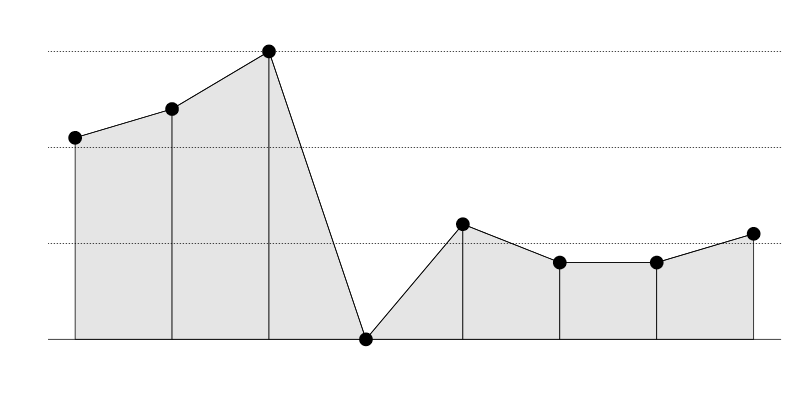
\includegraphics[width=0.48\textwidth]{graph/pipeline-23-1}
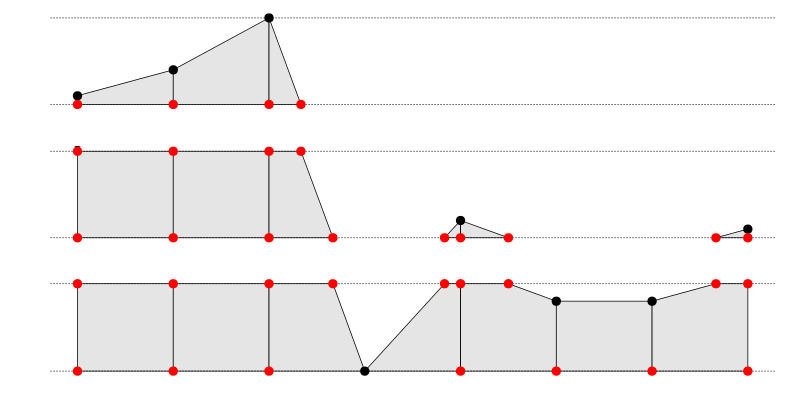
\includegraphics[width=0.48\textwidth]{graph/pipeline-23-2}
\end{centering}
\caption{\label{fig:Additional-data}Additional data created from the vertical
faceting. The black dots are given by the time series, and the red
dots are created during the cropping step of faceting.}
\end{figure}
\end{center}

\end{itemize}

\end{document}
